\section{Dataset Preparation}
Here, we will employ the event-related entries in Freebase~\cite{bollacker2008freebase} to automatically annotate event descriptions in Wikipedia's pages, with the essence of  \texttt{DS}. We regard a sentence as positive when it mentions the occurrence of an event, or otherwise negative. For example, S1 and S2 are positive examples with their arguments in italics and underlined (also shown in Figure~\ref{fig:3}), while S3 and S4 are negative.
\begin{quote}
	\textbf{S1}: \underline{\emph{Remedy Corp}} was sold to \underline{\emph{BMC Software}} as the \underline{\emph{Service Management Business Unit}} in \underline{\emph{2004}}.
\end{quote}
\begin{quote}
	\textbf{S2}: \underline{\emph{Microsoft}} spent \$6.3 billion buying online display advertising company \underline{\emph{aQuantive}} in \underline{\emph{2007}}.
\end{quote}
\begin{quote}
	\textbf{S3}: Microsoft hopes aQuantive's Brian McAndrews can outfox Google.
\end{quote}
\begin{quote}
	\textbf{S4}: On April 29th, Elizabeth II and Prince Philip witnessed the marriage of Prince William.
\end{quote}
%
\subsection{Freebase}
Freebase is a structured knowledge base, and there are three basics concepts: \emph{instance}, \emph{type} and \emph{property}. \emph{Instances} are entries in Freebase, and related to real-world entities and their relationships. \emph{Types} are different perspectives of \emph{instances}. \textbf{\emph{Compound Value Type}} (CVT) is a special type in Freebase to represent complex structured data where instances are described with multiple \textbf{\emph{properties}}, usually organized in a table. Some of the CVT schemas indeed imply certain events, e.g., \emph{people.marriage}, \emph{military.military\_service} and \emph{business.acquisition}, and closely resemble to event structures, where CVT properties can be treated as event arguments. As shown in Figure~\ref{fig:3}, 

the properties of CVT  \emph{business.acquisition}  actually can be used to label  %can be used to represent 
the participants and attributes of the events mentioned in S1 and S2.

We use the Freebase copy of 2013-06,  %version of Berant et al. \shortcite{berant2013semantic}, 
containing 1010 CVTs. After filtering out those %CVTs that 
describing the Freebase structures  or irrelevant to events (e.g., \emph{food.recipe\_ingredient}), we obtain 24 CVTs with around 280 million instances.    
%
\begin{figure}[h]
	\centering
	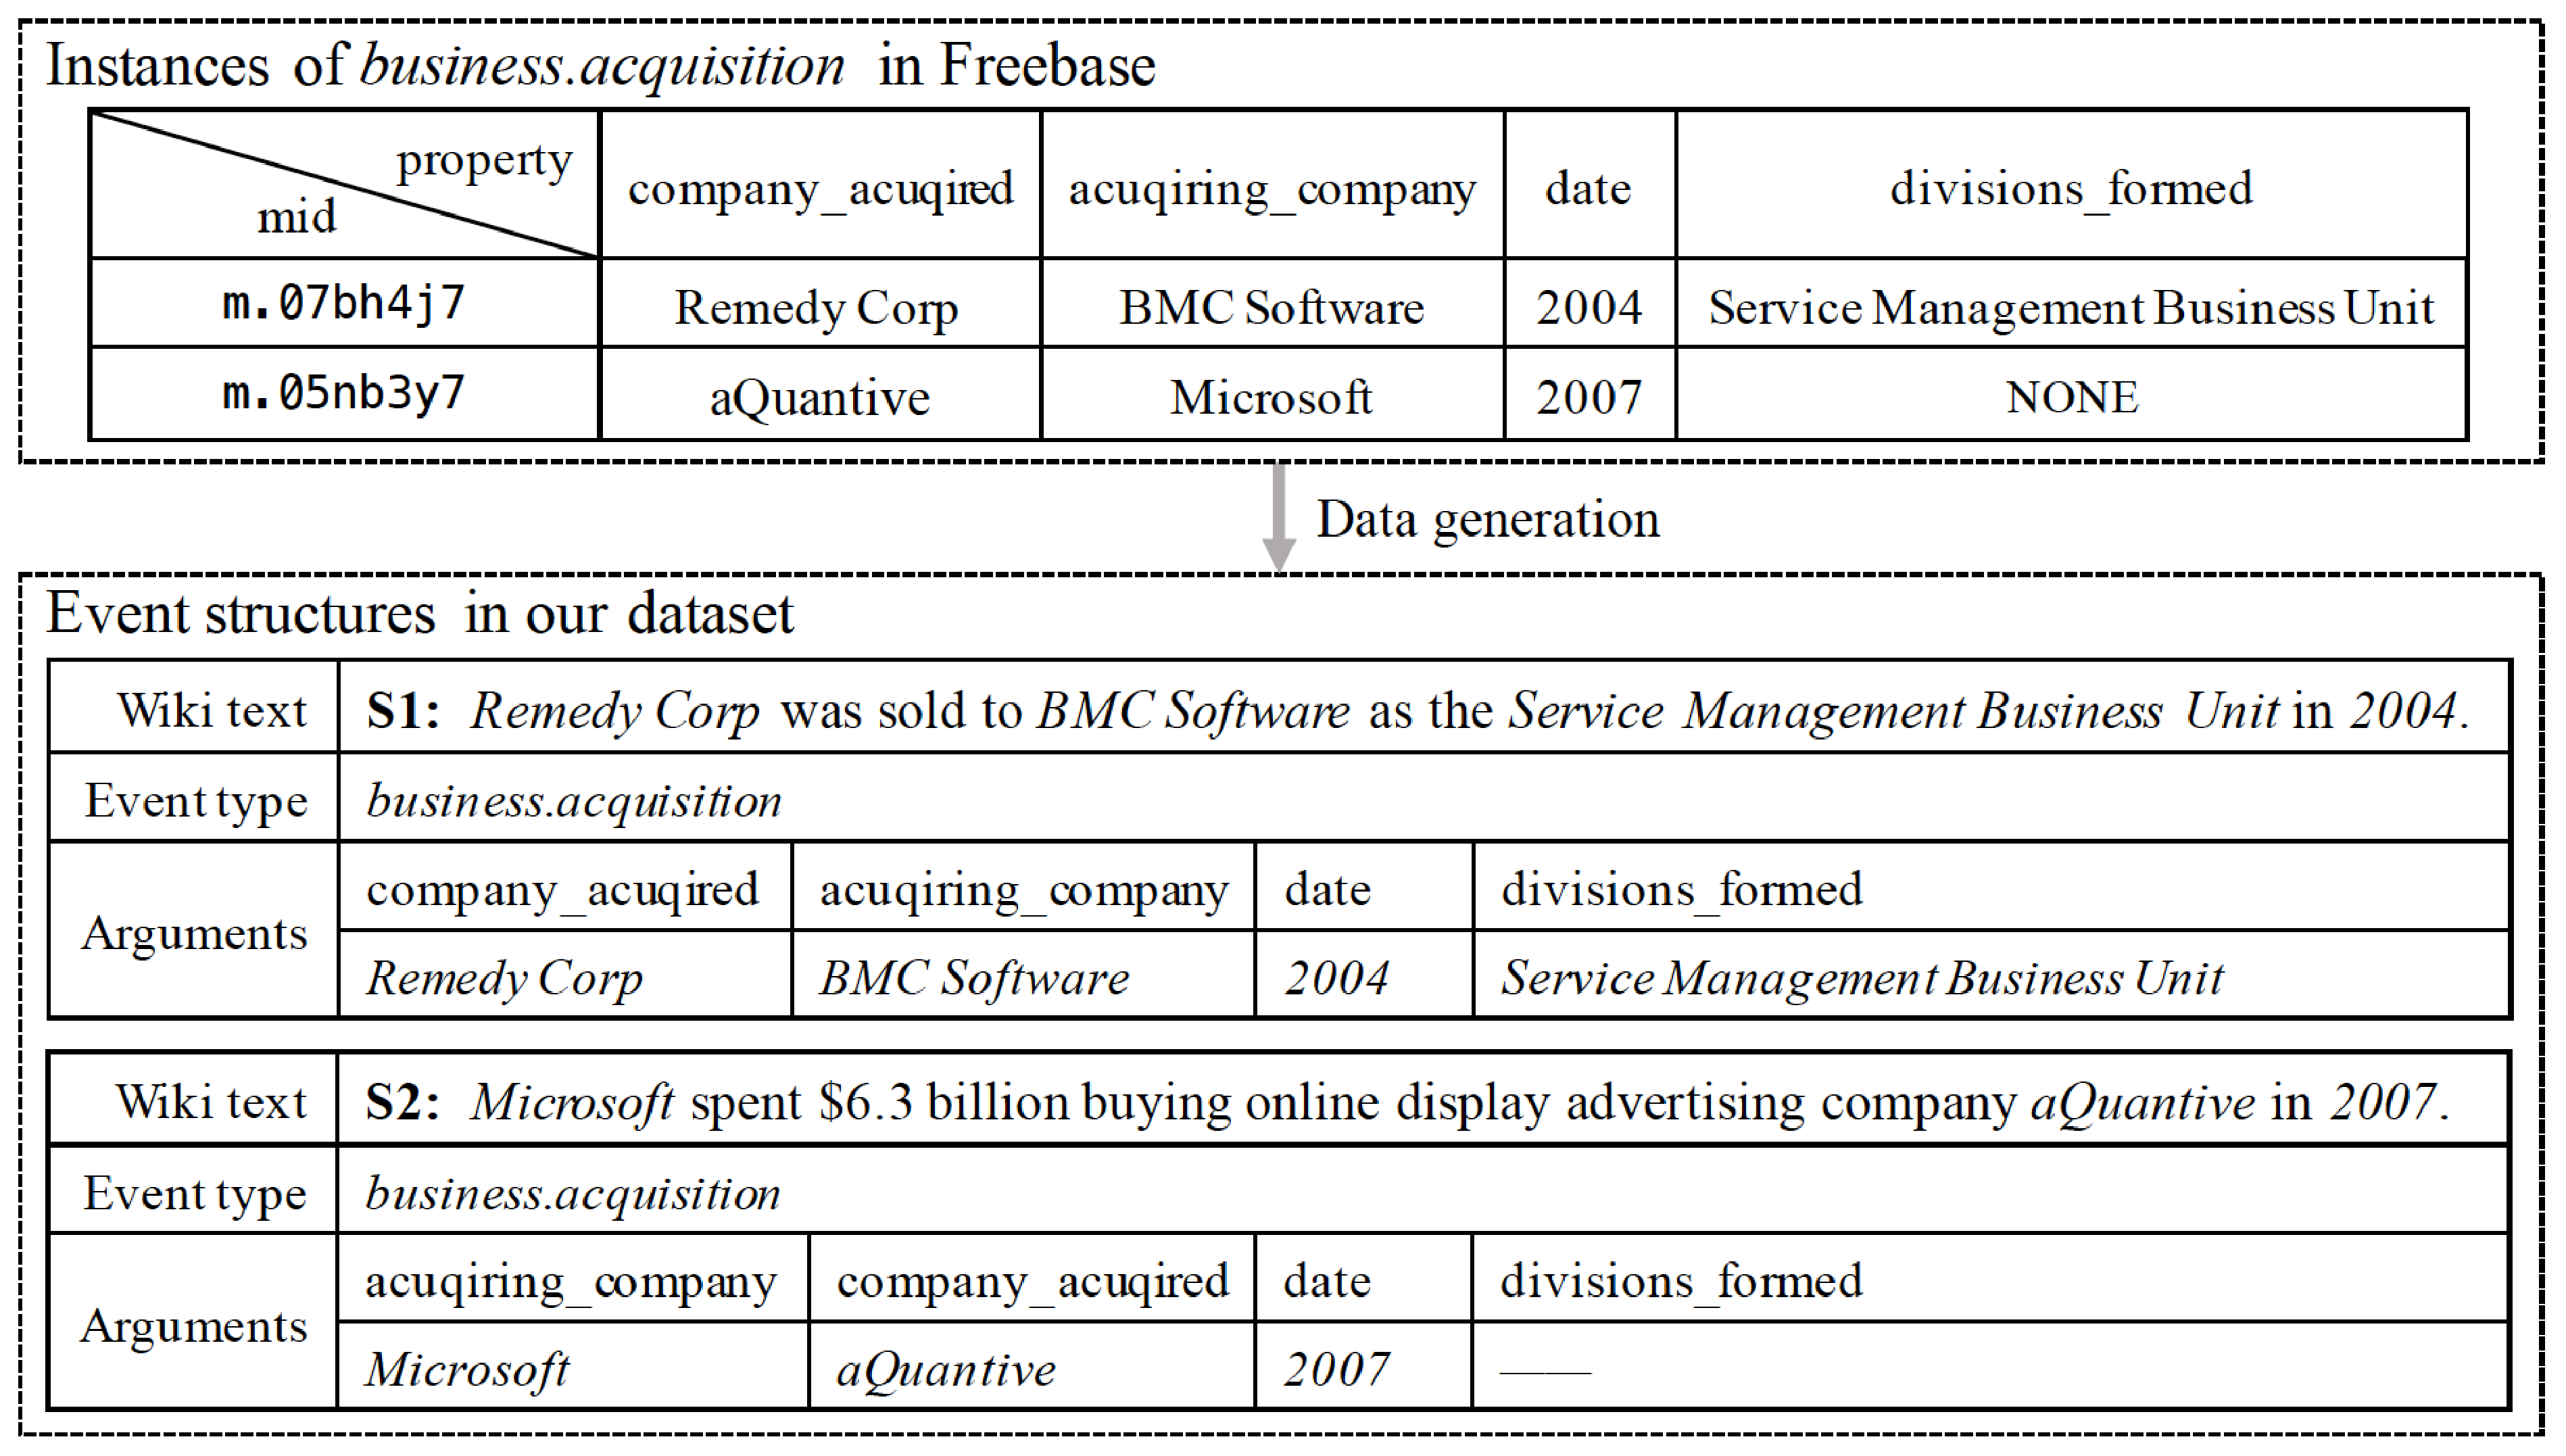
\includegraphics[width=.45\textwidth]{temp}
	\caption{Examples of CVT instances in Freebase, and labeled sentences in our dataset. \emph{Company\_acuqired}, \emph{acquiring\_company} and \emph{date} are key arguments in \emph{business.acquisition}. \label{fig:3}}
\end{figure}

\subsection{Data Generation\label{datagen}}
Now we will describe how to automatically collect training data with quality event annotations, by pushing forward the \texttt{DS} framework.
\subsubsection{H1: Positive sentences should contain all properties}
Our first hypothesis is that \textit{if a sentence contains all properties of an entry in a CVT, this sentence will be 
considered as a positive sample to indicate an event of such type characterized by this CVT}.  
We will then label the sentence as a mention of this CVT event, and the words or phrases that 
match this entry's properties as the involved arguments, with the roles specified by their 
corresponding property names. 
For example, S1 contains all the properties of instance $m.07bh4j7$ with a CVT type \emph{business.acquisition}, 
we thus consider S1 as a positive sample implying an event about \emph{business.acquisition}, and \emph{BMC Software}, \emph{Remedy Corp}, \emph{Service Management Business Unit} and \emph{2004} will be labeled as the arguments that play the role of \emph{acquiring\_company}, \emph{company\_acquired}, \emph{divisions\_formed}, and \emph{date} in this event, respectively.

%However, in practice, we realize that \emph{H1} is too strict that excludes a great many positive sentences like S2. 

\subsubsection{H2: Positive sentences should contain all key properties}
In practice, we find that \emph{H1} is too strict to include many positive sentences like S2. 
We thus relax \emph{H1} by replacing \textbf{all properties} with \textbf{all key properties}. We define the CVT property that plays an important part in its CVT structure and helps to distinguish with other CVTs as a \textbf{key property}. A \textbf{key argument} is the word/phrase that matches a key property of a CVT instance. For example, \emph{company\_acquired} and \emph{acquiring\_company} are the key properties of CVT \emph{business.acquisition}, therefore,  S2 should be a positive sentence for a \emph{business.acquisition} event, since it contains all key properties. Table~\ref{tab:5} lists the key properties of four CVTs.

The importance of a property $prop$ (e.g., \emph{date}) to its CVT $cvt$ (e.g., \emph{business.acquisition}) can be defined as:
\begin{equation}
	degree_{cvt, prop} = log \frac{count(cvt, prop)}{count(cvt) \times count(prop)} 
\end{equation}
where $count(cvt)$ is the number of all instances of type $cvt$, $count(prop)$ is the number of times $prop$ appearing in all CVTs, and $count(cvt, prop)$ is the number of $cvt$ instances that contain the property $prop$.

\begin{table}
\centering
\small
\begin{tabular}{|l|l|} \hline
CVT & Key properties \\ \hline
award.award\_honor & award\_winner, award, \ldots, year \\ \hline
film.performance & actor, film, character \\ \hline
education.education & institution, student, end\_date \\ \hline
business.employment\_tenure & company, title, person, from \\ \hline
\end{tabular}
\caption{Examples of key properties of four CVTs.\label{tab:5}}
\end{table}

\subsubsection{H3: Key properties should include time properties}
%We discover that for many CVTs, their key properties do not take into account time property. 
Although time-related arguments are often missing in the currently imperfect KBs, time-related properties are indeed
crucial to indicate an actual event mention, e.g., S3, containing  \emph{Microsoft} as \emph{acquiring\_company} and \emph{aQuantive} as \emph{company\_acquired} but without time-related arguments, will be considered as a positive sample for event \emph{business.accquisition} by mistake.
% while contain all key properties of an instance, resulting in mistaking \emph{Microsoft} for \emph{acquiring\_company}, and \emph{aQuantive} for \emph{company\_acquired}. 
%By adding \emph{date} to the set of key properties, S3 will be filtered. 
We thus include time-related properties with highest importance scores  as supplementary key properties. 

\subsubsection{H4: Key properties should be closer on dependency path}
%We introduce another factor, syntactic distance, to annotate positive instances.
Intuitively, two arguments participating in the same event are likely to be closer to each other in syntactic structures, which will help to eliminate negative samples. In Figure~\ref{fig:2},  both  \emph{Prince Philip} and \emph{marriage} can be matched as key properties in a \textit{people.marriage} entry,  but are far from each other on the dependency path, thus S4 should be labeled as negative.
%The distance can be measured by the distance of two words in dependency parsing tree. 
In our experiments, we set the maximum distance between two key arguments as 2.
%, i.e., for a candidate sentence, if a pair of key arguments violates this constraint, it is supposed to be negative. 
%Given the dependency parsing tree in Figure~\ref{fig:2}, S4 is negative because the distance between \emph{Prince Philip} and \emph{marriage} is 3.

\begin{figure}
\centering
	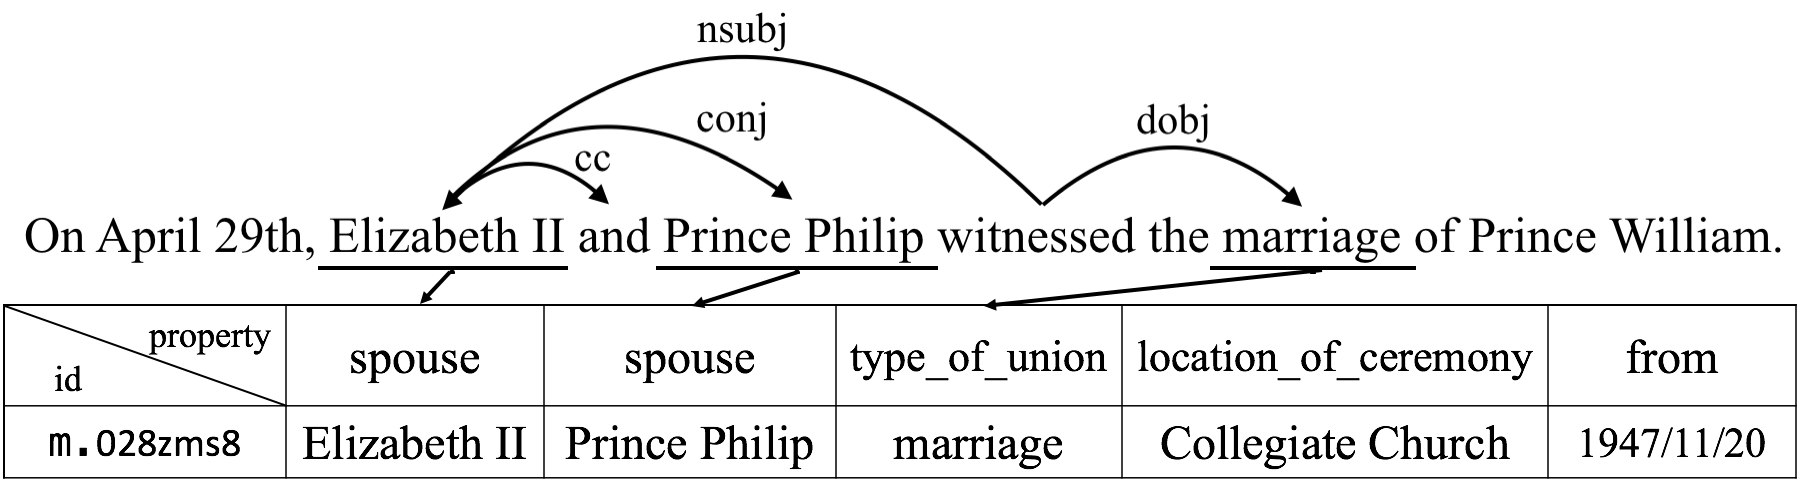
\includegraphics[width=.47\textwidth]{deppath}
	\caption{An illustration of dependency tree of S4, which partially matches an entry of \emph{people.marriage}. \label{fig:2}}
\end{figure}

We conduct a series of manual evaluations on the quantity and quality of the 
 datasets produced by different hypotheses (see Sec~\ref{sec:evalhypo}), 
and the combination of  \emph{H3} and \emph{H4} produces the best dataset, thus serves 
as our final strategy.
